\documentclass[10pt]{jarticle}
\usepackage{float}
\usepackage{adrobo_abst}
\usepackage[dvipdfmx]{graphicx}
\usepackage{amssymb,amsmath}
\usepackage{bm}
\usepackage[superscript]{cite}
\usepackage{enumerate}
\usepackage{url}
%\usepackage[absolute]{textpos}

\renewcommand\citeform[1]{(#1)}

\begin{document}
    
    \makeatletter
    \doctype{2024年度卒業論文概要}
    \title{視覚と行動のend-to-end学習により\\経路追従行動を模倣する手法の提案}{(経路選択の成功率向上を意図したネットワークの変更と実験的評価)}
    \etitle{A proposal for an imitation method of path-tracking behavior\\by end-to-end learning of vision and action}{(Modification of network aimed at improving route selection success rate and its experimental evaluation)}
    
    \author{21C1011\hspace{.5zw}石黒巧}
    \eauthor{Takumi ISHIGURO}
    
    \makeatother
    
    \abstract{
        Recent research explores navigation using camera images. 
        Okada et al. proposed end-to-end learning for path-following from metric maps, using visual input. 
        Haruyama et al. extended this by adding branching recognition from camera images and scenario-based path selection defined by Shimada et al.
        Experiments confirmed robots could visually follow paths to destinations. 
        However, Haruyama et al.'s tests were limited, with success in only 7 of 50 scenarios.
        This study examines autonomous navigation feasibility in untested scenarios using only camera images. To improve results, network enhancements and new training methods were implemented. 
        Tests in real-world environments confirmed successful navigation in previously unexplored scenarios. 
    }
    \keywords{autonomouse moblie robot, end-to-end learning, navigation}
    
    \maketitle
    
    \supervisor{指導教員: 林原靖男教授}
    
    \section{緒\hspace{2zw}言}%===========================
    近年,ロボットにおけるカメラ画像を用いたナビゲーションの研究が進んでいる.
    本研究室の岡田ら\cite{okada2020}はメトリックマップベースの経路追従行動を end-to-end 学習を用いて模倣学習することで,視覚に基づくナビゲーション手法を提案した.
    また,春山ら\cite{haruyama2023}はカメラ画像とシナリオに基づいて目的地まで経路追従するシステムを提案した.
    % シナリオとは島田らが提案した,「条件」と「行動」に関する単語を組みわせて構成されている.
    この手法は岡田らの手法をベースに,カメラ画像から通路の種類を分類し,シナリオに基づいて経路を選択する機能を追加した.
    % 春山らは、島田が作成した 50 例のシナリオから 7 例を選定している。
    春山らは,島田ら\cite{Shimada2020}が作成したシナリオから 7 例を選定し,目的地まで到達できることを確認した.
    選定外のシナリオは,地面の色が異なる場所や広場を含んでおり,視覚に基づいて経路追従するのがより困難な環境と考えられる.
    
    本論文では,島田らが作成したシナリオの中で,春山らが検証していないシナリオについて,目的地まで経路追従できるかを確認する.
    また,経路追従の成功率を向上させるための改良も行う.
    \section{視覚に基づいて目的地まで\\経路追従するシステム}
    春山らの手法\cite{haruyama2023}の概要を\reffig{system}に示す.
    システムは,
    % \vspace{-2.5zh}
    \begin{enumerate}
        \setlength{\parskip}{0cm} % 段落間
        \setlength{\itemsep}{0cm} % 項目間
        \item シナリオを分解し,「条件」と「行動」を抽出するシナリオモジュール
        \item カメラ画像と目標方向を与えることで,経路を追従する経路追従モジュール
        \item カメラ画像から通路の特徴を分類する通路分類モジュール
    \end{enumerate}
    の 3 つから構成される.
    まずは人間が目的地に応じた「条件」と「行動」から構成されるシナリオを作成する.
    シナリオからシナリオモジュールが行動を抽出し,経路追従モジュールが行動を実行する.
    通路分類モジュールが条件の達成を検出すると,次の行動に遷移する.
    \begin{figure*}[t]
        \centering
        \vspace{-1.5zh}
        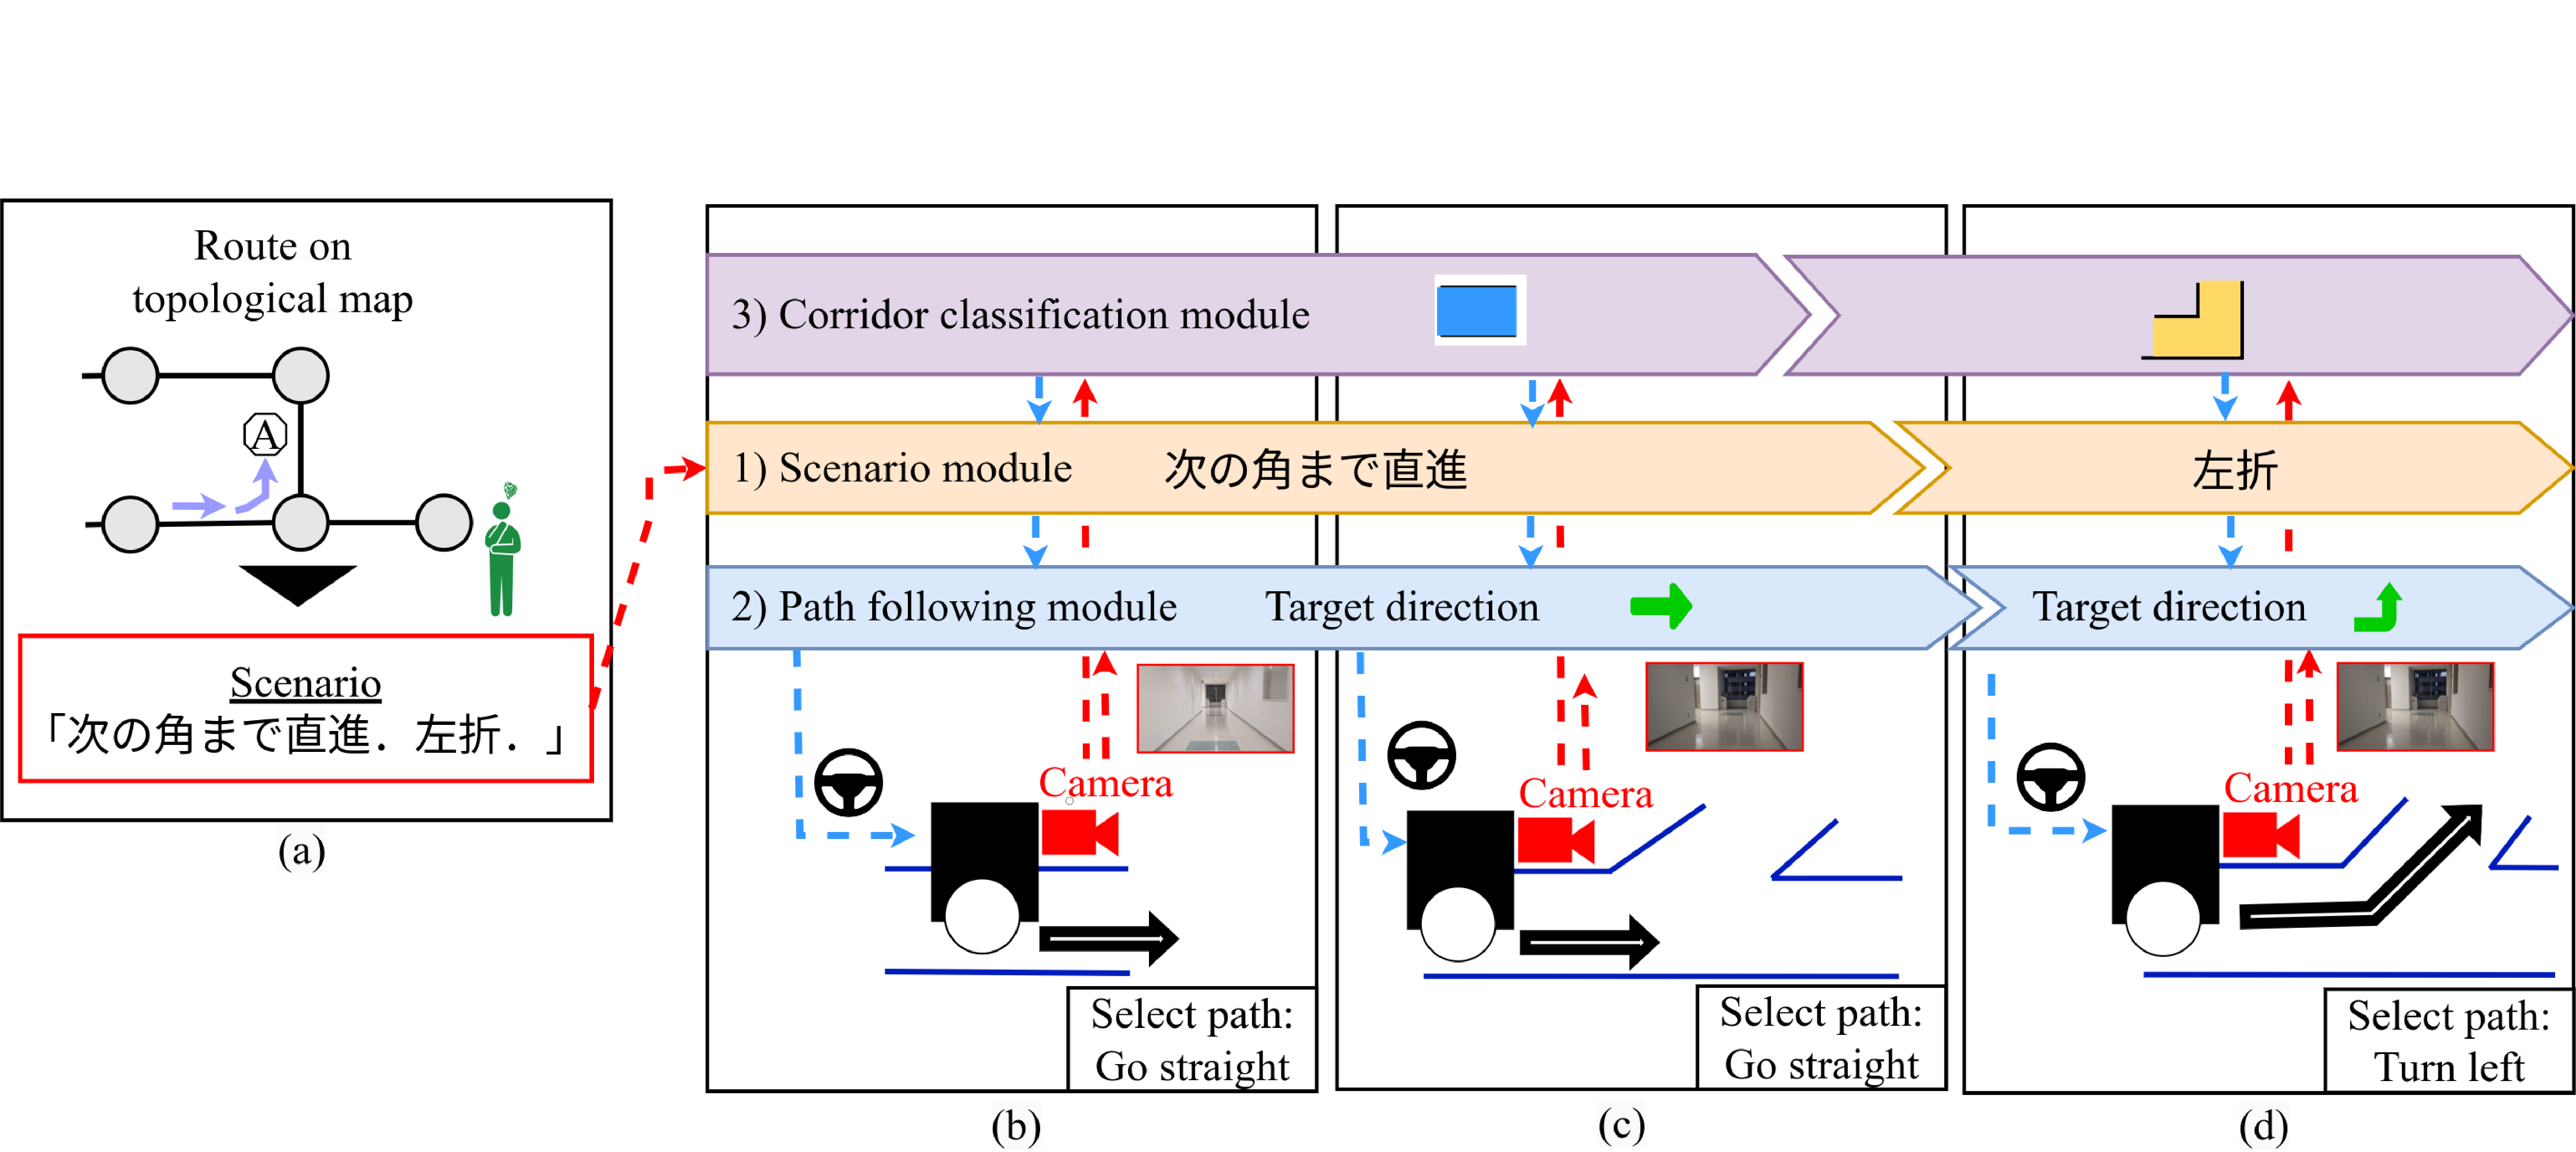
\includegraphics[width=105mm]{./fig/haruyama/system.pdf}
        \vspace{-1zh}
        \caption{Overview of proposed system by haruyama and others(Quoted from \cite{haruyama2023})}
        \label{fig:system}
    \end{figure*}

    % ロボットは下記の a から d の一連の流れにより,指示された経路に沿って目的地まで自律移動する.
    % \begin{enumerate}
    %     \setlength{\parskip}{0cm} % 段落間
    %     \setlength{\itemsep}{0cm} % 項目間
    %     \item [(a)] 目的地に応じた「条件」と「行動」のシナリオを人間が作成.
    %     \item [(b)] シナリオモジュールが「条件」と「行動」を抽出し、初めの行動を経路追従モジュールに指示
    %     \item [(c)] 通路分類モジュールが条件達成を検出し、シナリオモジュールが次の行動へ遷移を判断
    %     \item [(d)] 経路追従モジュールが次の行動を実行
    % \end{enumerate}


    \section{機能の改善}%===========================
    経路追従モジュールに関して,経路追従の可能性を向上させるために以下の2点を変更した.
    \subsection{ネットワークの変更}
    % Felipeらの先行研究\cite{Codevilla2018}によると,目標方向などのコマンドによってモデルを分岐する形式のネットワークが,春山らが使用していた形式より経路追従の成功率が高いと報告している.
    Felipeら\cite{Codevilla2018}は,目標方向によってモデルを切り替えるネットワークを用いることで,経路追従の成功率を高められると報告している.
    そのため,Felipeらの形式を基に,\reffig{branched}に示すネットワークを構築した.
    ネットワークの入力は春山らと同様, RGB 画像と目標方向で,出力はロボットのヨー方向の角速度である.
    % 損失関数や活性化関数などのパラメータは春山らの手法と同様である.
    \vspace{-1zh}
    \begin{center}
        \begin{figure}[h]
            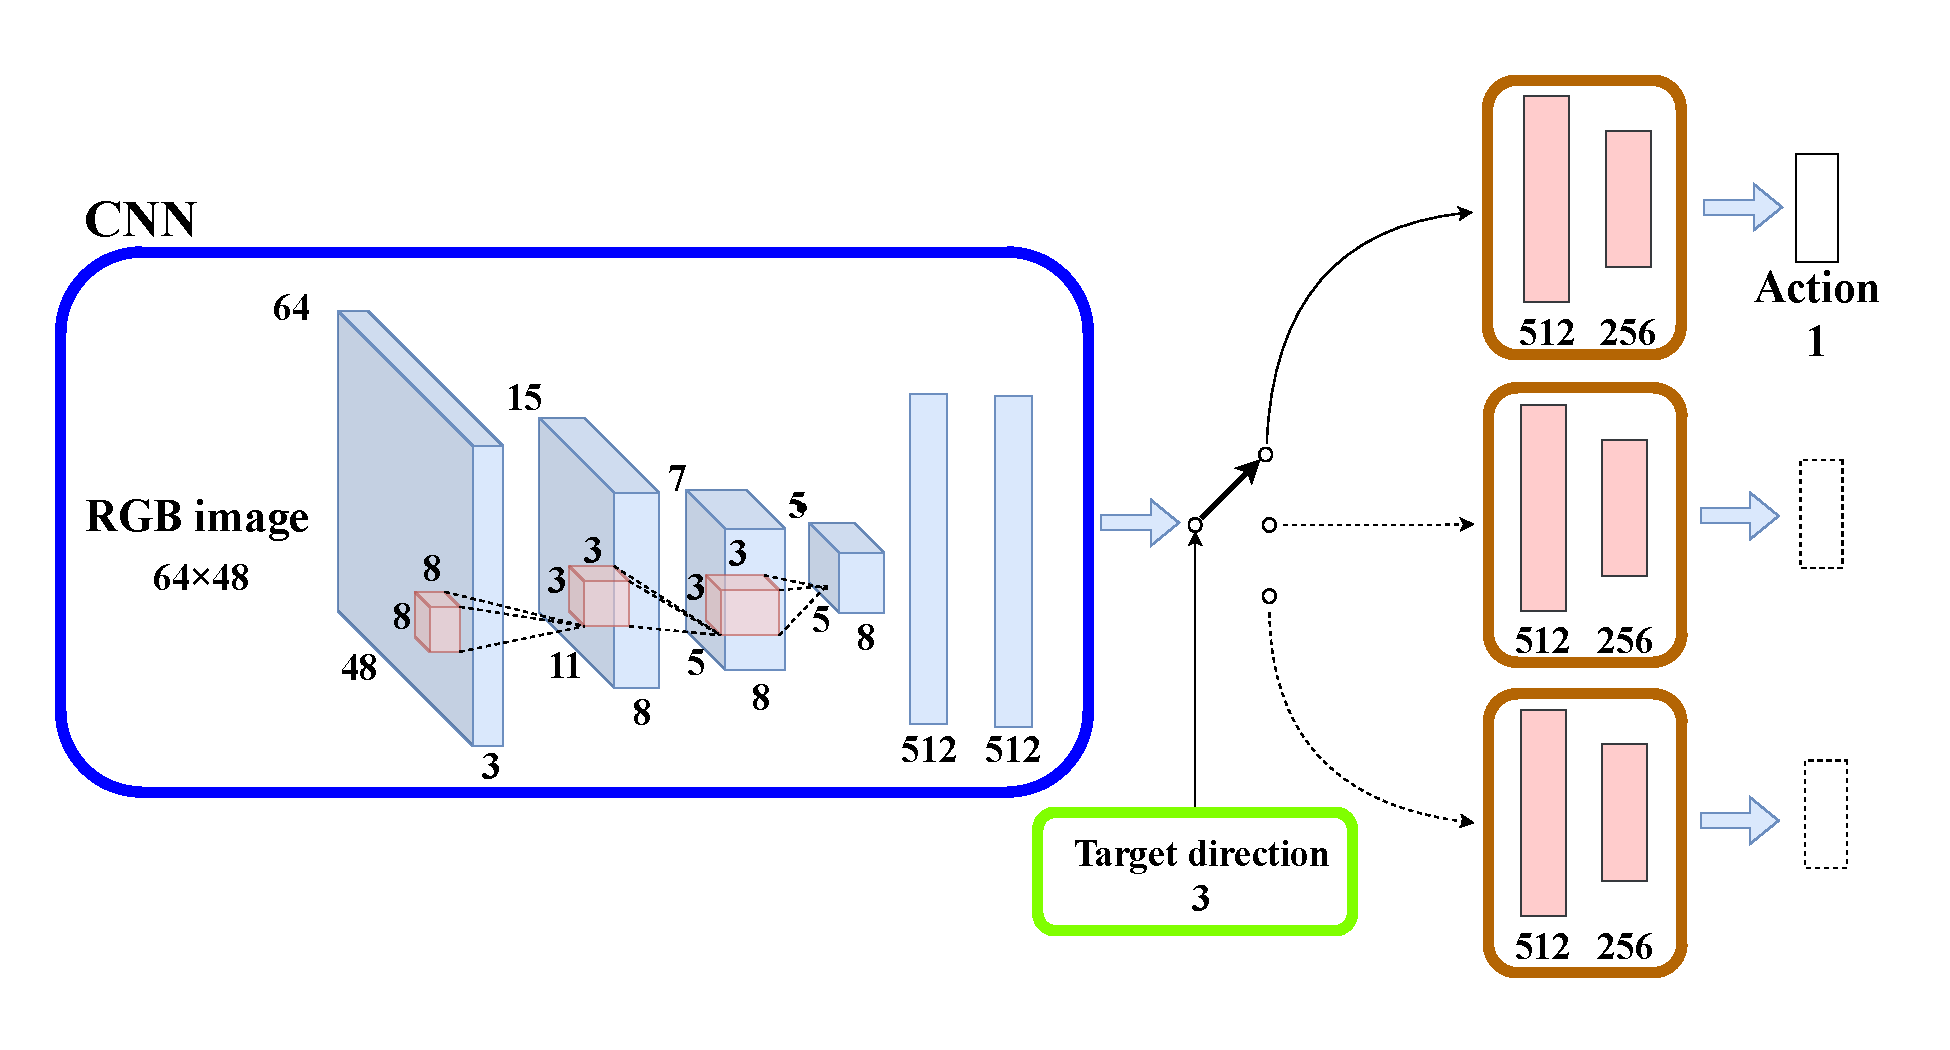
\includegraphics[width=0.475\textwidth]{./fig/ishiguro/branched.pdf}
            \vspace{-2zh}
            \caption{Branched network}
            \label{fig:branched}
        \end{figure}
    \end{center}
    \vspace{-3zh}

    \subsection{オフライン学習の併用}
    春山らの研究では,取得したデータを逐次学習するオンライン学習を用いていた.
    オンライン学習の問題点として,後半に取得したデータの学習回数が減少することで,走行できない箇所が生じることがある.
    この問題を解決するために,オフライン学習を併用する.
    ここでオフライン学習とはオンライン学習の際に作成したデータセットを使用して追学習することを指す.


    \section{実\hspace{2zw}験}%===========================
    春山らが未検証のシナリオに関しても,ロボットが目的地へ到達可能であるか検証する.
    \subsection{実験装置}
    \reffig{gamma}に実験に使用するロボットを示す.
    
    \begin{figure}[h]
        \centering
        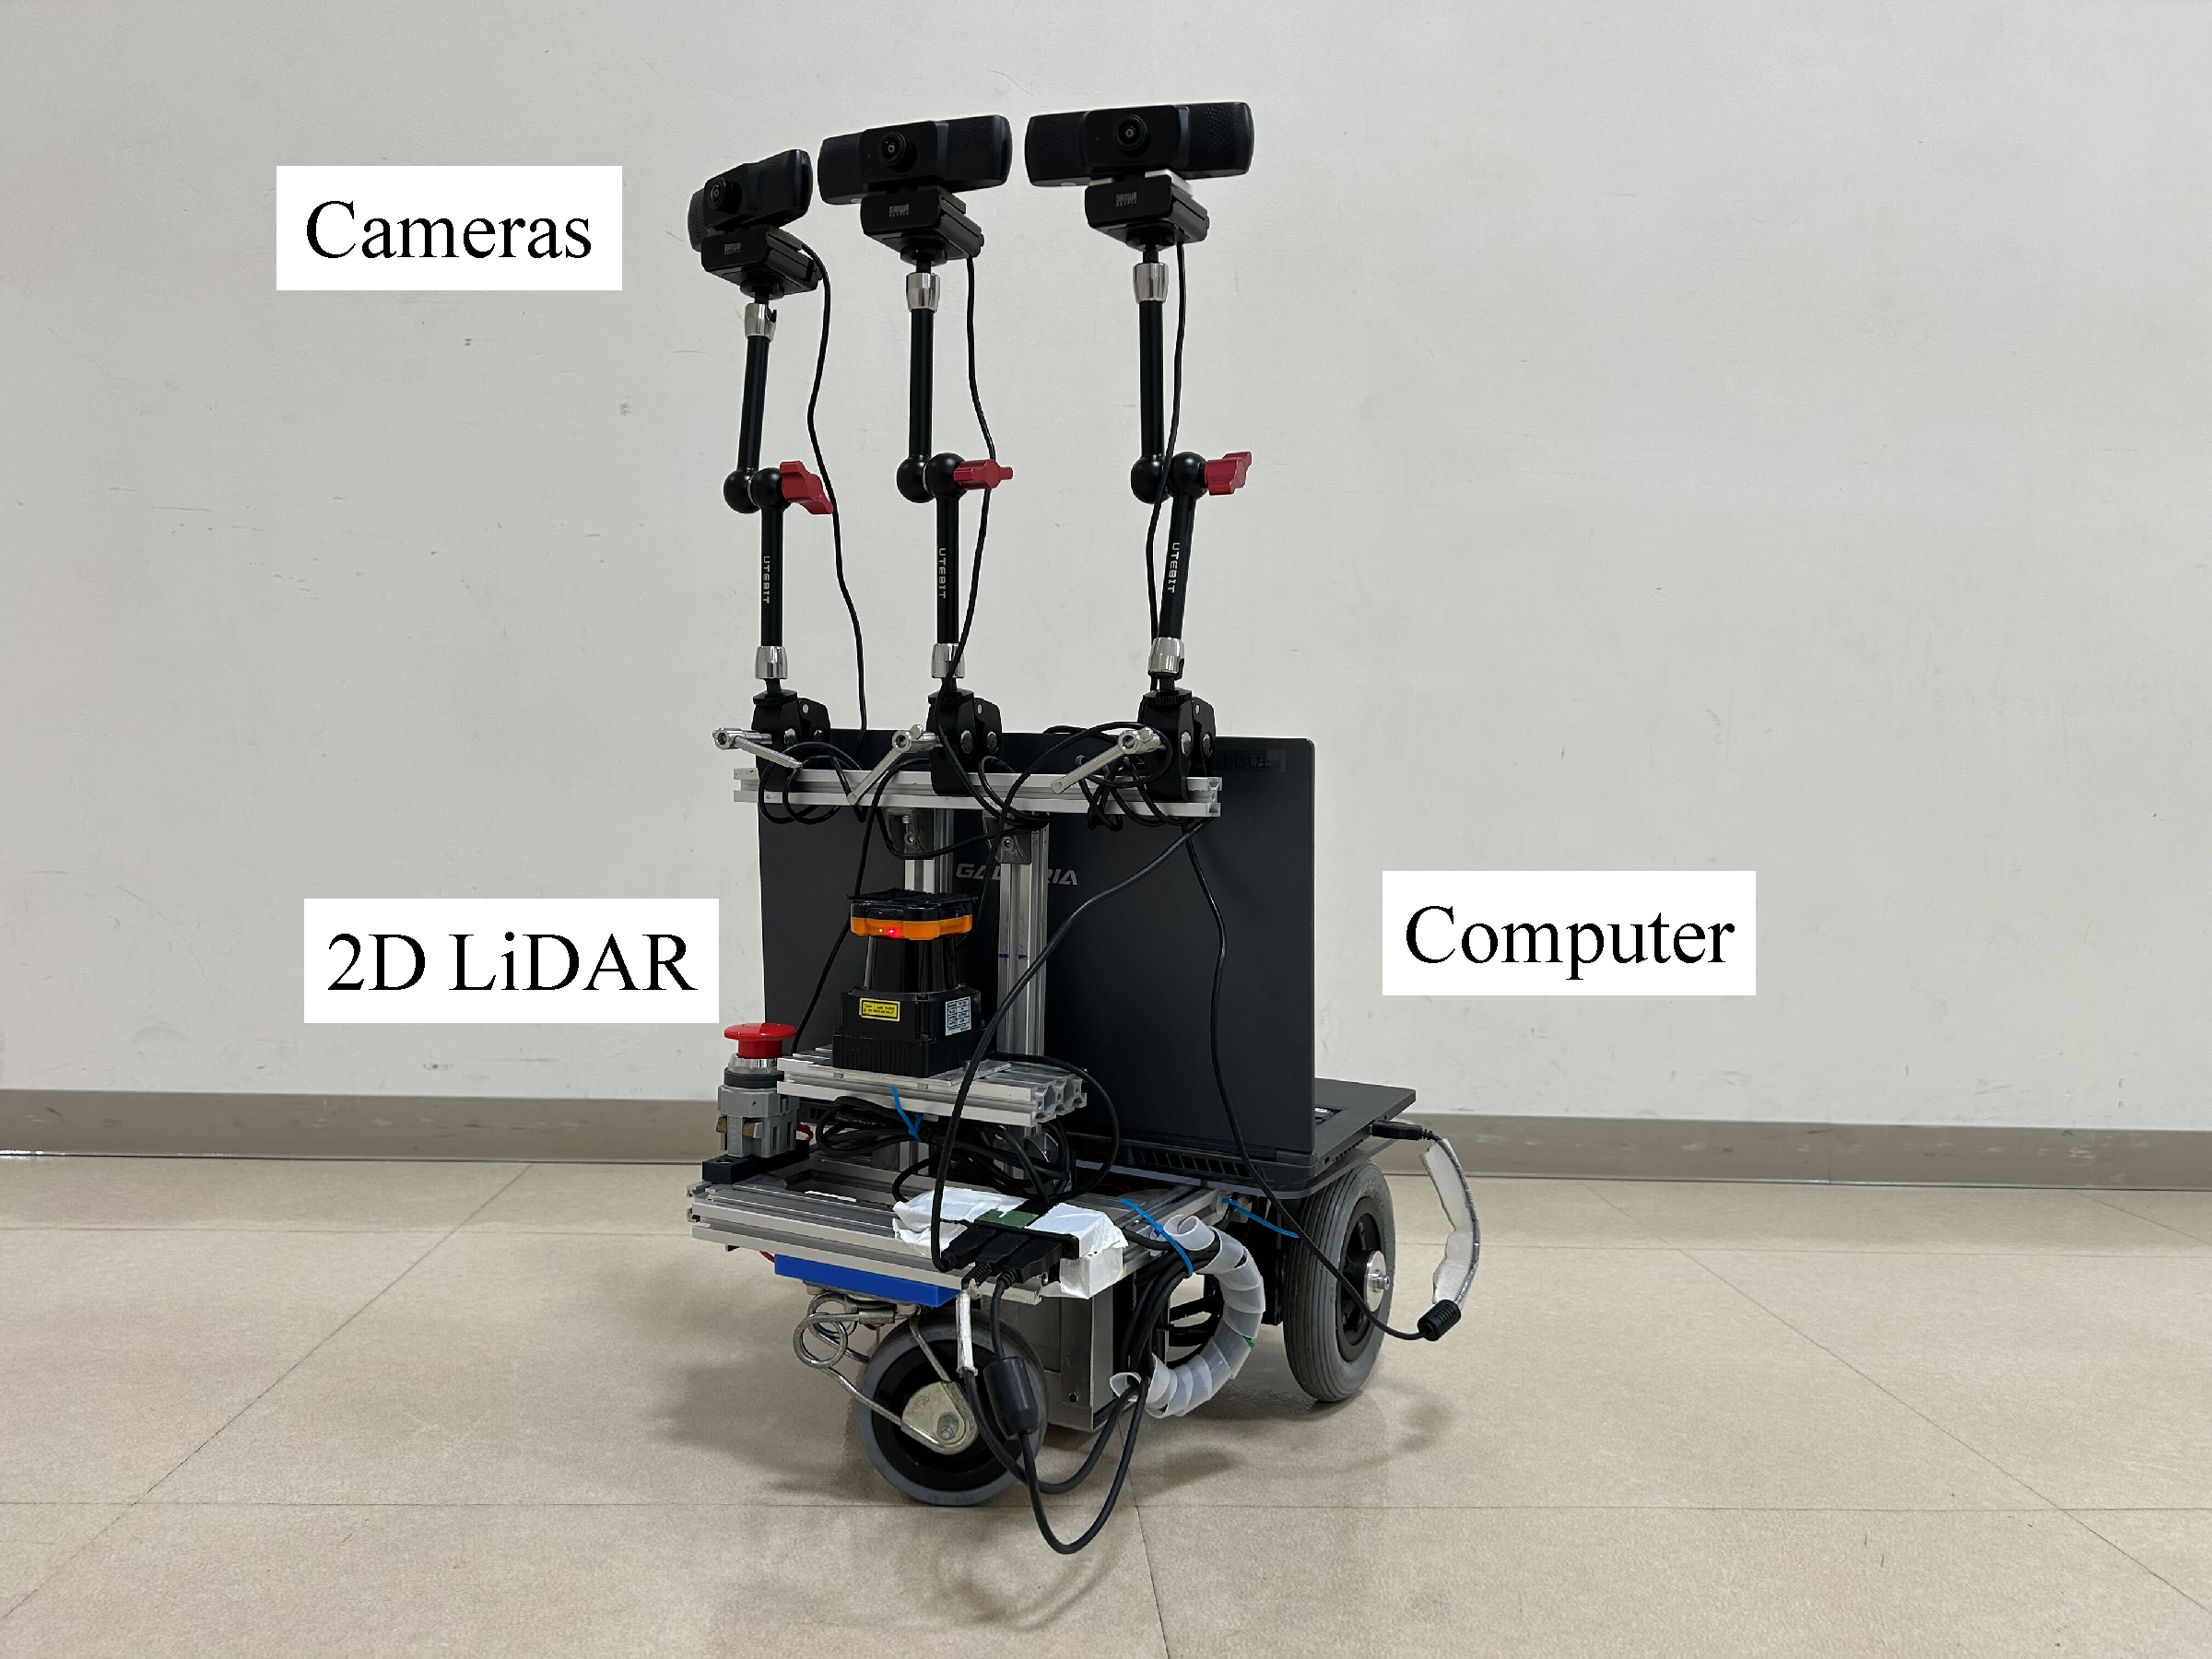
\includegraphics[width=0.25\textwidth]{./fig/ishiguro/gamma.pdf}
        \vspace{-1zh}
        \caption{Experimental setup}
        \label{fig:gamma}
    \end{figure}
    
    \subsection{実験方法}
    % \begin{center}
    %     \begin{figure}[!b]
    %         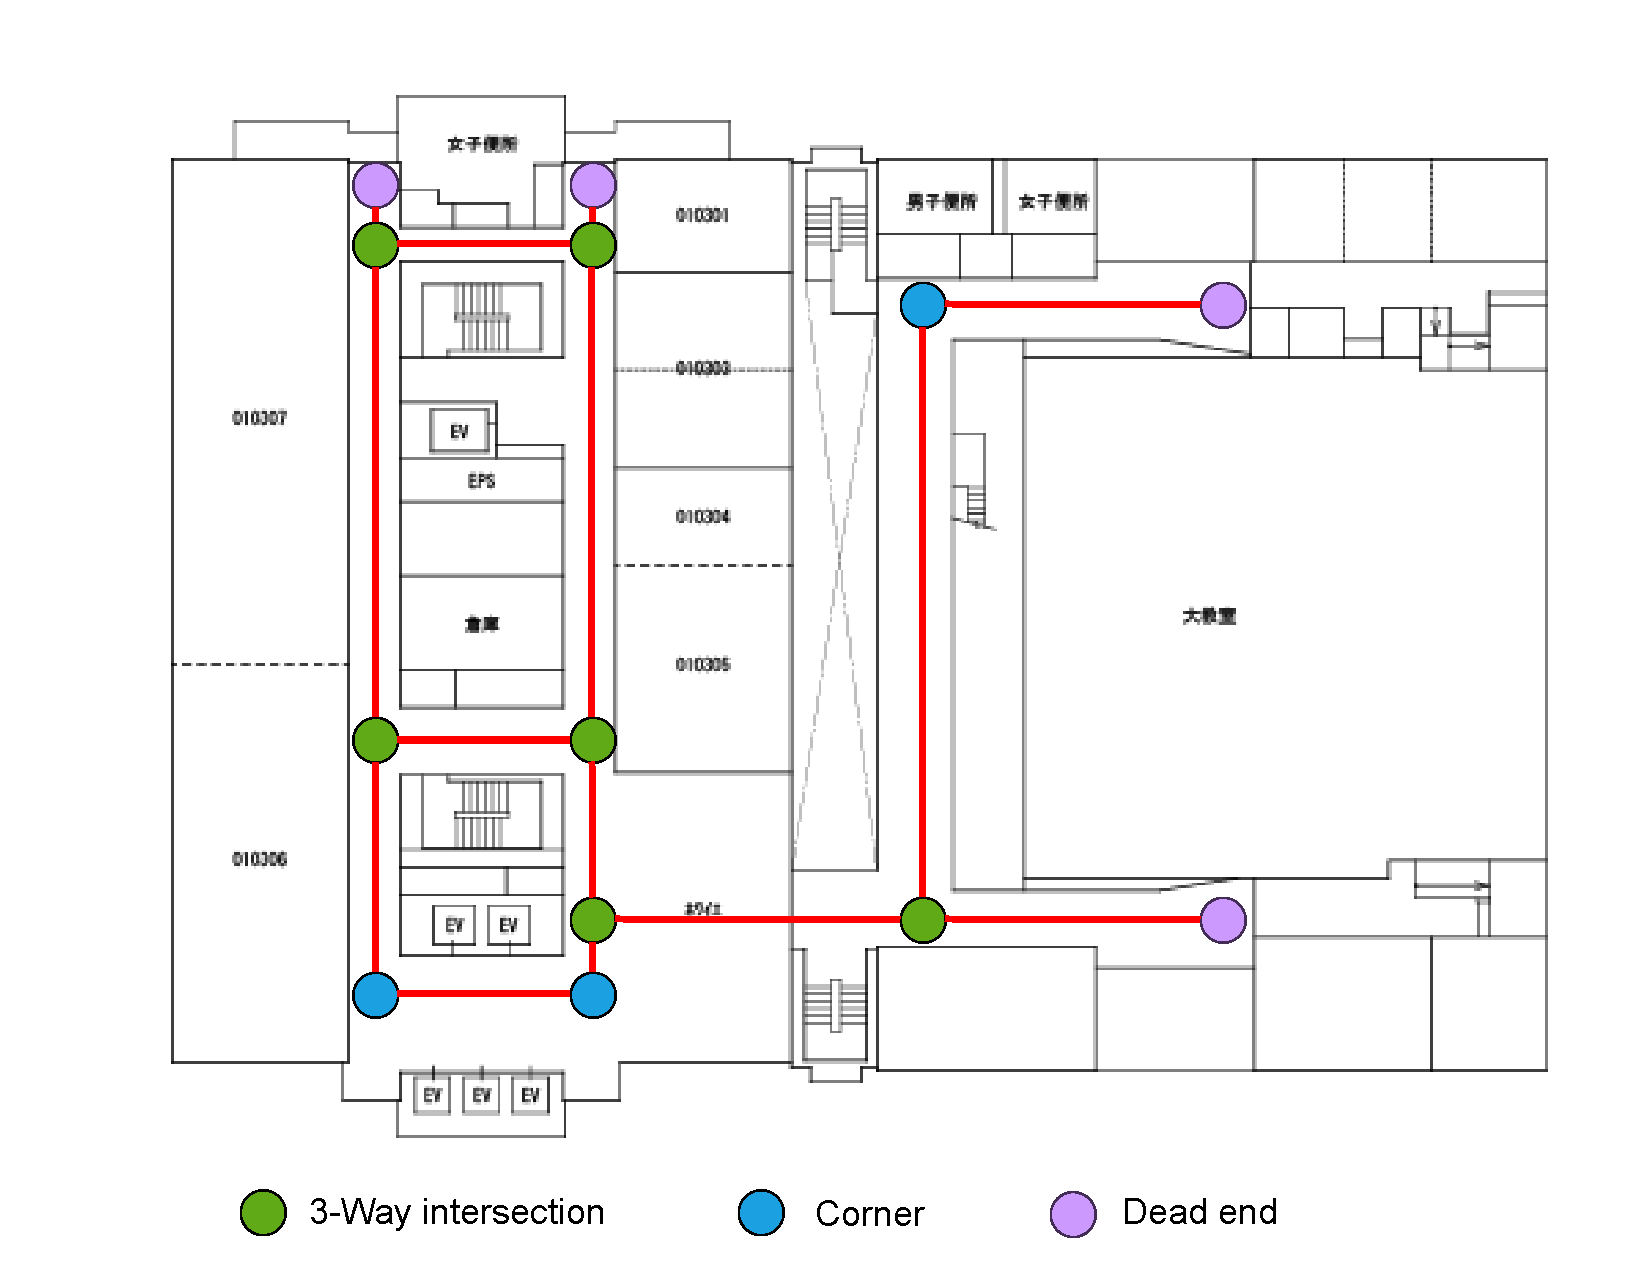
\includegraphics[width=0.45\textwidth]{./fig/ishiguro/topo.pdf}
    %         \caption{aaaaaaaaaaaa}
    %         \label{fig:route}
    %     \end{figure}
    % \end{center}
    実験環境として千葉工業大学津田沼キャンパス 2 号館 3 階を用いる.
    訓練時にはオンライン学習を行いながら,ルートを 1 周走行する.
    次に作成したモデルに追加でオフライン学習を行う.   
    % \subsubsection{通路分類モジュールの訓練}
    % % \figref{fig:route}に示すルートをROS の navigation パッケージを使用して,経路を 1 周する.
    % その際, 3 つのカメラからそれぞれ画像データを収集しながら走行する.
    % 学習時のパラメータとして,バッチサイズを 32 ,epoch数を 30 とした.

    訓練後,ロボットが目的地まで到達できるか確認する.
    ロボットをシナリオのスタート地点,向きに配置し,シナリオを 1 例ずつ入力する.
    壁に衝突することなく指定した経路を選択し,目的地で停止した場合に成功とする.

    \subsection{実験結果}
    シナリオ 28 例中,24 例の成功を確認した.
    失敗は,曲がるべき角で,直進したことがその要因である.
    原因として,通路分類モジュールの出力に遅れがあることが挙げられる.
    解析の結果,経路追従モジュールへ目標方向を与えるタイミングが遅いため,曲がらずに直進することを確認した.

    \section{結\hspace{2zw}言}%===========================
    本論文では,経路追従の成功率を向上させるためにネットワークの変更,オフライン学習を行った.
    春山らの先行研究では走行が確認されていないシナリオでも目的地まで経路追従できることを確認した.


    \vspace{5truemm}
    {\footnotesize
        \begin{thebibliography}{99}
            
            \bibitem{okada2020}
            岡田眞也 , 清岡優祐 , 上田隆一 , 林原靖男 .
            ``視覚と行動の end-to-end 学習により経路追従行動をオンラインで模倣する手法の提案'',
            計測自動制御学会 SI 部門講演会 SICE-SI2020予稿集 , 
            pp.1147-1152(2020).

            \bibitem{haruyama2023}
            春山健太 , 藤原柾 , 馬場琉生 , 石黒巧 , 上田隆一 , 林原靖男 .
            ``視覚と行動のend-to-end学習により経路追従行動をオンラインで模倣する手法の提案 -トポロジカルマップとシナリオに基づく経路選択機能の追加と検討-'',
            計測自動制御学会 SI 部門講演会 SICE2023 予稿集,
            pp.1B4-03(2023).
       
            \bibitem{Codevilla2018}
            F. Codevilla, M. Müller, A. López, V. Koltun, A. Dosovitskiy: 
            ``End-to-end Driving via Conditional Imitation Learning'', 
            arXiv preprint, arXiv:1710.02410 (2018), 
            \url{https://arxiv.org/abs/1710.02410}.

            \bibitem{Shimada2020}
            島田滉己,上田隆一,林原靖男,
            ``トポロジカルマップを用いたシナリオによるナビゲーションの提案 -シナリオに基づく実ロボットのナビゲーション-'',
            計測自動制御学会 SI 部門講演会 SICE2020 予稿集,
            pp.1H2-04(2020).



        \end{thebibliography}
    }
    \normalsize
    
\end{document}
